%%%%%%%%%%%%%%%%%%%%%%%%%%%%%%%%%%%%%%%%%%
% a0poster Portrait Poster
% LaTeX Template
% Version 1.0 (22/06/13)
%
% The a0poster class was created by:
% Gerlinde Kettl and Matthias Weiser (tex@kettl.de)
% 
% This template has been downloaded from:
% http://www.LaTeXTemplates.com
%
% License:
% CC BY-NC-SA 3.0 (http://creativecommons.org/licenses/by-nc-sa/3.0/)
%
%%%%%%%%%%%%%%%%%%%%%%%%%%%%%%%%%%%%%%%%%

%----------------------------------------------------------------------------------------
%	PACKAGES AND OTHER DOCUMENT CONFIGURATIONS
%----------------------------------------------------------------------------------------

\documentclass[a0,portrait]{a0poster}

\usepackage{multicol} % This is so we can have multiple columns of text side-by-side
\columnsep=100pt % This is the amount of white space between the columns in the poster
\columnseprule=3pt % This is the thickness of the black line between the columns in the poster

\usepackage[svgnames]{xcolor} % Specify colors by their 'svgnames', for a full list of all colors available see here: http://www.latextemplates.com/svgnames-colors

\usepackage{times} % Use the times font
%\usepackage{palatino} % Uncomment to use the Palatino font

\usepackage{graphicx} % Required for including images
\graphicspath{{figures/}} % Location of the graphics files
\usepackage{booktabs} % Top and bottom rules for table
\usepackage[font=small,labelfont=bf]{caption} % Required for specifying captions to tables and figures
\usepackage{amsfonts, amsmath, amsthm, amssymb} % For math fonts, symbols and environments
\usepackage{wrapfig} % Allows wrapping text around tables and figures
\usepackage[latin1]{inputenc}
%\usepackage[lmargin=3cm,rmargin=3cm,tmargin=3cm,bmargin=3cm]{geometry}
\usepackage[latin1]{inputenc}
\usepackage{indentfirst}

\usepackage{setspace,cite}
\onehalfspacing

\renewcommand\refname{Bibliografia}
\renewcommand\figurename{Figura}

\usepackage{array}

\begin{document}

%----------------------------------------------------------------------------------------
%	POSTER HEADER
%----------------------------------------------------------------------------------------

% The header is divided into two boxes:
% The first is 75% wide and houses the title, subtitle, names, university/organization and contact information
% The second is 25% wide and houses a logo for your university/organization or a photo of you
% The widths of these boxes can be easily edited to accommodate your content as you see fit

\begin{minipage}[b]{1.0\linewidth}
\center
\veryHuge \color{Black} \textbf{Controle e Simula\c{c}\~ao de Sistemas Sujeitos a Saltos Markovianos} \color{Black}\\ % Title
\Huge \textbf{Oscar Neiva E.~Neto}\\ % Author(s)
{\huge\textbf{{\em orientador:}\, Marcos G.~Todorov, D.~Sc.}}\\ % Author(s)
\huge Laborat\'orio Nacional de Computa\c{c}\~ao Cient\'ifica - LNCC\\
\huge Faculdade de Educa\c{c}\~ao Tecnol\'ogica do Estado do Rio de Janeiro - FAETERJ\\
%Coordena\c{c}\~ao de Sistemas e Controle - CSC\\[.4em] % University/organization
\Large \texttt{oscarnen@lncc.br\qquad todorov@lncc.br}\\
\end{minipage}
%

%\vspace{1cm} % A bit of extra whitespace between the header and poster content

%----------------------------------------------------------------------------------------

\begin{multicols}{2} % This is how many columns your poster will be broken into, a portrait poster is generally split into 2 columns


%%%%%%%%%%%%%%%%%%%%%%%%%%%%%%%%%%%%%%%%%%%%%%%%%%%%%%%%%%%%%%%%%%%%%%%%%%%%%%%%
%\begin{abstract}
%Este trabalho \'e dedicado ao estudo de sistemas sujeitos a saltos markovianos e quest\~oes relacionadas a cadeias de \textit{Markov}. A partir da leitura de artigos publicados, que despertaram interesse da comunidade de sistemas e controle, pode-se guiar os estudos de sistemas estoc\'asticos por meio de implementa\c{c}\~oes computacionais.
%\end{abstract}
%%%%%%%%%%%%%%%%%%%%%%%%%%%%%%%%%%%%%%%%%%%%%%%%%%%%%%%%%%%%%%%%%%%%%%%%%%%%%%%%

\vspace{1cm}

%----------------------------------------------------------%
\section{Introdu\c{c}\~ao}
%----------------------------------------------------------%

Este trabalho \'e dedicado ao estudo de sistemas sujeitos a saltos Markovianos e quest\~oes relacionadas a cadeias de Markov. A pesquisa desenvolvida visa o aprendizado de aspectos te\'oricos fundamentais relacionados a cadeias de Markov, teoria de controle, e simula\c{c}\~ao de problemas distribu\'idos.\\[-2em]

%----------------------------------------------------------%
\section{Sistemas Lineares com Saltos Markovianos}
%----------------------------------------------------------%

Considere $\theta = \{\theta(k), k = 0,1,\ldots\}$ uma cadeia de Markov homog\^enea no espa\c{c}o de estados discreto $\mathbf{N} = \{1,2,...,M\}$, isto \'e, tal que:
%
\begin{equation}
P \bigl( \theta(k+1) = j \mid  \theta(k) = i, \theta(k-1),
   \ldots, \theta(0)\bigr)
= P \bigl( \theta(k+1) = j \mid  \theta(k) = i\bigr),
\end{equation}
%
que \'e denominada a propriedade de Markov. Tal processo estoc\'astico tem aplica\c{c}\~ao em diversas \'areas da ci\^encia como, por exemplo, computa\c{c}\~ao, engenharia, economia e biologia \cite{bremaud}.

O interesse neste trabalho \'e no estudo de sistemas din\^amicos governados pela seguinte equa\c{c}\~ao:
%
\begin{equation} \label{xAB}
	x(k+1) = A_{\theta(k)} x(k),\qquad k=0,1,2,\ldots,
\end{equation}
%
onde $x$ \'e o estado do sistema. Existe uma vasta literatura dedicada ao estudo desses sistemas, que sofrem varia\c{c}\~oes abruptas em sua estrutura. Uma amostra significativa de avan\c{c}os recentes pode ser encontrada no livro \cite{costafragosotodorov}.\\[-2em]

%----------------------------------------------------------%
\section{PageRank}
%----------------------------------------------------------%

O \textit{PageRank} foi criado em 1998 para atribuir valores para p\'aginas de um conjunto de documentos interligados \cite{pagerankSIREV}. A ideia por tr\'as do algoritmo \'e de atribuir pesos \`as p\'aginas da \textit{world wide web}, em que recebem os maiores pesos as mais visitadas.\\[-2em]

%----------------------------------------------------------%
\subsection{Defini\c{c}\~ao}
%----------------------------------------------------------%

A an\'alise do PageRank tipicamente modela a web como um grafo orientado contendo $N$ n\'os, que representam as p\'aginas, e uma cole\c{c}\~ao de arestas $\mathcal{E}$ que representam os links correspondentes. A navega\c{c}\~ao \'e ent\~ao representada atrav\'es de uma cadeia de Markov com espa\c{c}o de estados discreto de dimens\~ao $N$. A hip\'otese usual \'e de que todas as arestas que saem de um dado n\'o t\^em o mesmo peso, e portanto a matriz de transi\c{c}\~ao da cadeia de Markov \'e a seguinte:
%
\begin{equation}
p_{ij} = \begin{cases}
\dfrac{1}{N_i}, & \text{caso}\, (i,j)\in \mathcal{E},\\
0, & \text{caso contr\'ario},
\end{cases}
\end{equation}
%
onde $N_i$ \'e o n\'umero de \textit{links} que saem da p\'agina $i$.

O PageRank de um conjunto de $N$ p\'aginas da web \'e definido como o vetor $x \in \mathbb{R}^{N \times 1}$ que satisfaz as seguintes equa\c{c}\~oes:
%
\begin{equation}	
	x = Ax, \quad x\geq0, \quad \sum^{N}_{j=1} x_{j} = 1, 
\end{equation}
%
onde $A \in \mathbb{R}^{N \times N}$ \'e a transposta da matriz de transi\c{c}\~ao da cadeia de Markov.

Um m\'etodo usual para obten\c{c}\~ao do PageRank \'e o chamado \textit{Power Method} \cite{ishiiMag14}, que busca aproximar o PageRank atrav\'es da seguinte itera\c{c}\~ao: $x(k+1) = Ax(k),\: k\geq0,\: \text{com} \: x(0) = x_0,$ onde $x_0 \in \mathbb{R}^{N \times 1}$ \'e uma condi\c{c}\~ao inicial positiva de soma igual a um.\\[-2em]

%----------------------------------------------------------%
\subsection{Teleportation Model}
%----------------------------------------------------------%

Muito embora a simplicidade do \textit{Power Method} o torne atraente, em geral ele n\~ao fornece uma garantia de converg\^encia. O \textit{Teleportation Model} \'e uma estrat\'egia reconhecida para que, atrav\'es de uma pequena modifica\c{c}\~ao na matriz $A$, o m\'etodo convirja globalmente para o PageRank. Matematicamente o \textit{teleportation model} \'e representado como uma combina\c{c}\~ao convexa de duas matrizes. Em que, $m$ \'e um par\^ametro, tal que $m \in (0,1)$, e a matriz link modificada \'e dada por $M \in \mathbb{R}^{N \times N}$, definida por, $M = (1-m)A + \frac{m}{n} 11^T,$ onde $11^T \in \mathbb{R}^{N \times N}$ \'e a matriz cujas entradas s\~ao todas iguais a um.\\[-2em]

%----------------------------------------------------------%
\subsection{Algoritmos Distribu\'idos}
%----------------------------------------------------------%

A fim de tornar o c\'alculo do PageRank menos custoso, e melhor explorar os recursos computacionais dos servidores dispon\'iveis na web, uma alternativa \'e o emprego de algoritmos distribu\'idos. A agrega\c{c}\~ao de tais experimentos aleat\'orios faz ent\~ao com que o \textit{power method} se torne um sistema linear com saltos Markovianos do seguinte tipo:
%
\begin{equation}
	x(k+1) = A_{\theta(k)}x(k), \quad k\geq0, \quad \text{com} \quad x(0) = x_0. 
\end{equation}

Para as matrizes links distribu\'idas $A_i \in \mathbb{R}^{N \times N}, \: i = 1,2, ..., n,$ tem-se que elas s\~ao definidas da seguinte forma: a i-\'esima coluna de $A_i$ coincide com a i-\'esima coluna de $A$, a j-\'esima entrada diagonal de $A_i$ \'e igual a um, para $j = 1, ..., n, \: j \neq i$, todas as outras entradas $a_{ij}$ s\~ao iguais a zero.

De forma similar ao que ocorre no \textit{power method}, este m\'etodo pode apresentar problemas de converg\^encia, que s\~ao resolvidos pela seguinte modifica\c{c}\~ao no \textit{teleportation model},
%
\begin{equation}\label{xA}
	x(k+1) = (1 - \hat{m})A_{\theta(k)}x(k) + \frac{\hat{m}}{N}11^T, \quad k \geq 0, \quad \text{com} \quad x(0) = x_0,
\end{equation}
%
onde  $\hat{m}$ \'e definido em atrav\'es da seguinte f\'ormula: $\hat{m} = \frac{2m}{n-m(n-2)}.$

Esse algoritmo converge, conforme mostrado em \cite{ishiiMag14}, no sentido da m\'edia quadr\'atica dada por: $\lim_{x\rightarrow \infty} \mathbb{E} [\parallel y(k)-x \parallel^2] = 0,$ onde $y(k)$ \'e a m\'edia do conjunto de amostras $x(0),... , x(k)$ definida como: $y(k) = \frac{1}{k+1} \sum_{l=0}^{k} x(l).$ Essa m\'edia \'e conhecida como m\'edia de Polyak ou m\'edia de C\`esaro e sua forma recursiva \'e dada por: $y(k+1) = \frac{(k+1)}{(k+2)}y(k) + \frac{1}{(k+2)}x(k+1).$\\[-2em]

%----------------------------------------------------------%
\section{Simula\c{c}\~oes}
%----------------------------------------------------------%

As simula\c{c}\~oes foram feitas considerando-se um conjunto de quatro p\'aginas, ou seja, uma cadeia de Markov com quatro estados. Foram feitas simula\c{c}\~oes dos tr\^es modelos descritos anteriormente, e uma simula\c{c}\~ao usando-se algoritmo de Monte Carlo.
%
\begin{center}
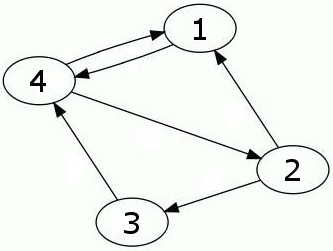
\includegraphics[width=9.4cm]{graph}
\end{center}

Na simula\c{c}\~ao do modelo do PageRank em sua forma mais simples, observa-se uma r\'apida converg\^encia para cada um dos valores do vetor de estados, isso ocorre devido a dimens\~ao do problema usado na simula\c{c}\~ao. 
%
Nesta simula\c{c}\~ao as linhas do gr\'afico est\~ao associadas \`as p\'aginas da seguinte forma: p\'agina 1 ao azul escuro, p\'agina 2 ao verde, p\'agina 3 ao vermelho e p\'agina 4 ao azul claro.
%
Assim pode-se observar que a p\'agina de n\'umero quatro foi a que recebeu um maior peso neste conjunto de links. Ao mesmo tempo que \'e a p\'agina que est\'a associada a um maior n\'umero de links, tanto de entrada quanto de sa\'ida.
%
\begin{center}
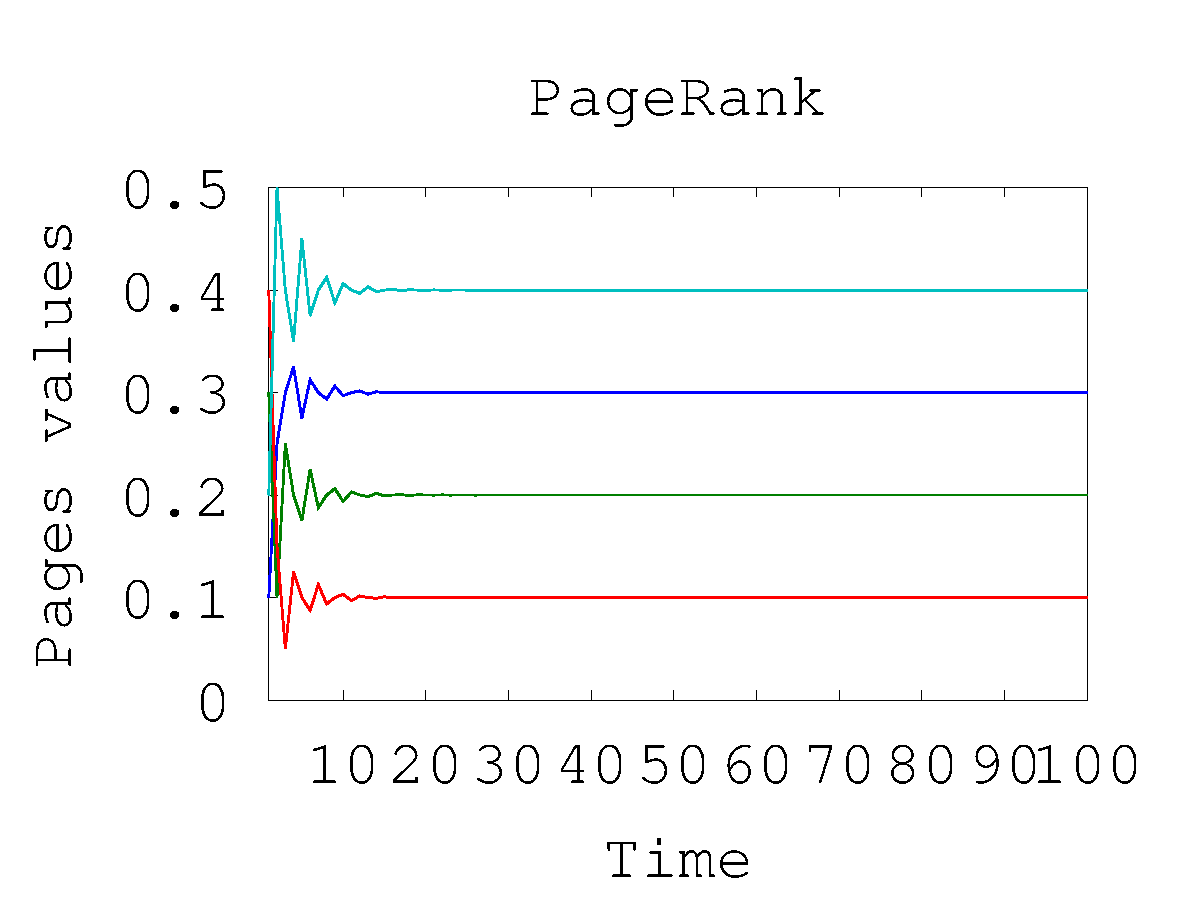
\includegraphics[width=.37\columnwidth]{pagerank.pdf}
\end{center}

Na simula\c{c}\~ao do \textit{Teleportation Model}, obteve-se uma grande semelhan\c{c}a com os resultados da simula\c{c}\~ao anterior, isso ocorre pois o exemplo simulado \'e bem comportado.

No modelo distribu\'ido observa-se uma oscila\c{c}\~ao dos estados sem que ao longo do tempo estacionem em algum valor, mas feita a m\'edia dos valores da cadeia no modelo distribu\'ido, chega-se a valores finais pr\'oximos aos anteriormente encontrados para cada um dos estados. 
%
Ao final fez-se uma simula\c{c}\~ao usando m\'etodo de Monte Carlo, de forma que \'e feita uma m\'edia dos estados obtidos na simula\c{c}\~ao do modelo distribu\'ido.
%
\begin{center}
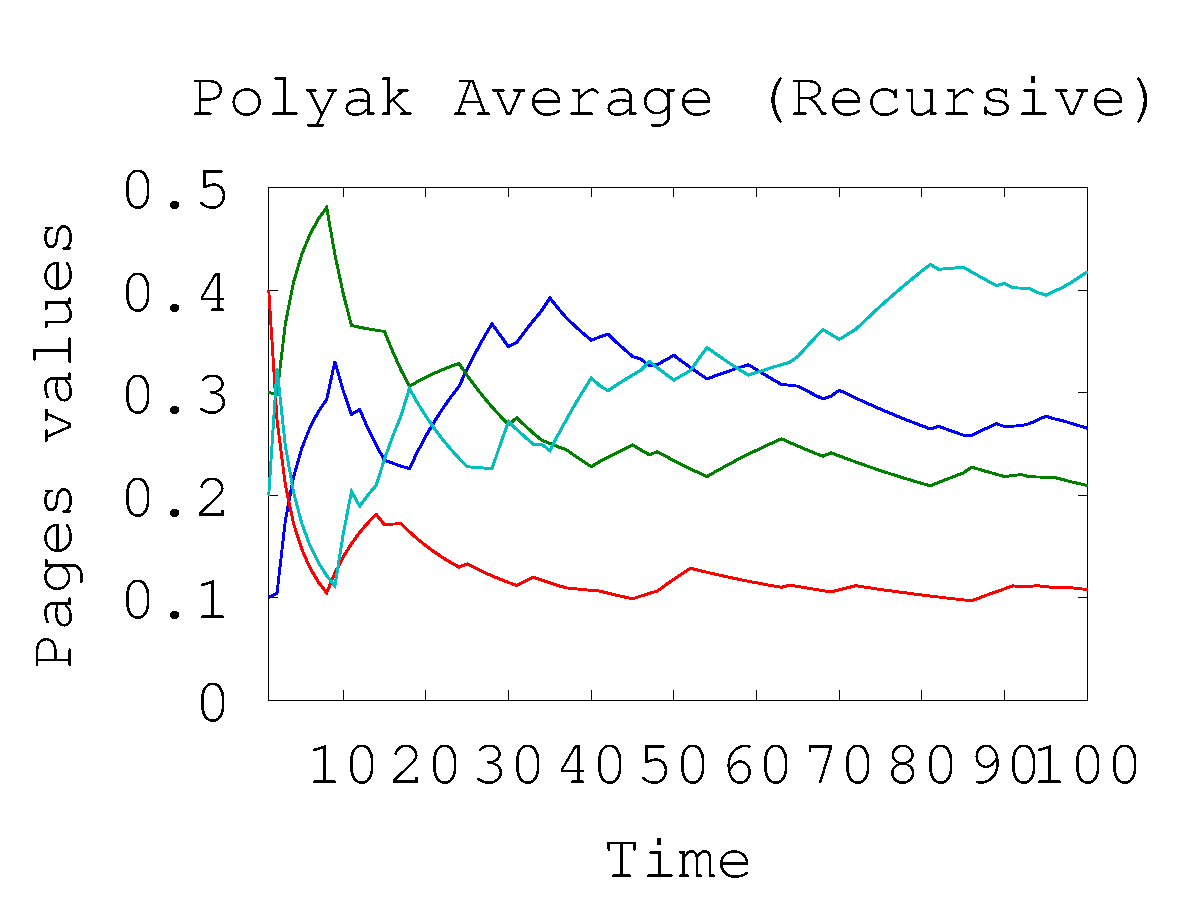
\includegraphics[width=.37\columnwidth]{polyakrecursive}
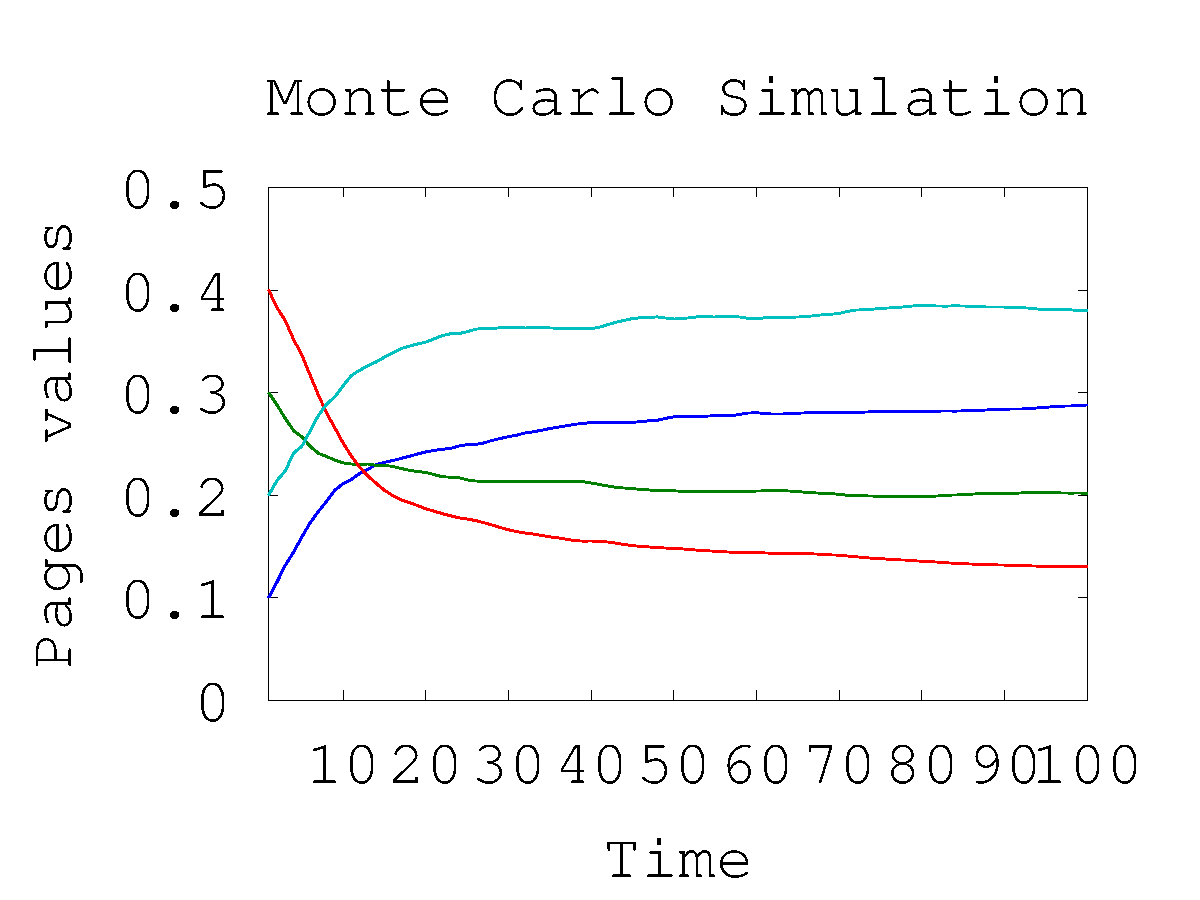
\includegraphics[width=.37\columnwidth]{montecarlo}
\end{center}
\vspace{-2cm}
%----------------------------------------------------------%
\section{Perspectivas Futuras}
%----------------------------------------------------------%

Neste projeto pretende-se ainda trabalhar com outros m\'etodos de controle e simula\c{c}\~ao de sistemas estoc\'asticos, que tamb\'em sejam v\'alidos na simula\c{c}\~ao do PageRank. Simula\c{c}\~oes essas como as de modelos agregados de cadeias de Markov e dentro do contexto do PageRank abordagens tamb\'em de problemas de consenso.\\[-2em]

%\vspace{1cm}

%----------------------------------------------------------------------------------------
%\bibliographystyle{plain}
%\bibliography{ref}


\begin{thebibliography}{1}

\bibitem{bremaud}
P.~Br\'emaud.
\newblock {\em Markov Chains: {G}ibbs Fields, {M}onte {C}arlo Simulation, and
  Queues}, volume~31 of {\em Texts in Applied Mathematics}.
\newblock Springer, New York, 1999.

\bibitem{pagerankSIREV}
K.~Bryan and T.~Leise.
\newblock The \$25,000,000,000 eigenvector: The linear algebra behind {G}oogle.
\newblock {\em SIAM Rev.}, 48(3):569--581, 2006.

%\bibitem{costafragosomarques}
%O.~L.~V. Costa, M.~D. Fragoso, and R.~P. Marques.
%\newblock {\em Discrete-Time {Markov} Jump Linear Systems}.
%\newblock Probability and Its Applications. Springer-Verlag, New York, 2005.

\bibitem{costafragosotodorov}
O.~L.~V. Costa, M.~D. Fragoso, and M.~G. Todorov.
\newblock {\em Continuous-Time {Markov} Jump Linear Systems}.
\newblock Probability and Its Applications. Springer-Verlag, Heidelberg, 2013.

%\bibitem{ishiiSCL12}
%H.~Ishii, R.~Tempo, and E.-W. Bai.
%\newblock Page{R}ank computation via a distributed randomized approach with
 % lossy communication.
%\newblock {\em Systems Control Lett.}, 61:1221--1228, 2012.

%\bibitem{ishiiTAC10}
%H.~Ishii and R.~Tempo.
%\newblock Distributed randomized algorithms for the {P}age{R}ank computation.
%\newblock {\em {IEEE} Trans. Automat. Control}, 55(9):1987--2002, 2010.

\bibitem{ishiiMag14}
H.~Ishii and R.~Tempo.
\newblock The {P}age{R}ank problem, multiagent consensus, and web aggregation:
  a systems and control viewpoint.
\newblock {\em IEEE Control Syst. Mag.}, 34(3):34--53, 2014.

%\bibitem{weiren}
%W.~Ren and R.~W. Beard.
%\newblock {\em Distributed Consensus in Multi-Vehicle Cooperative Control:
%  Theory and Applications}.
%\newblock Communications and Control Engineering. Springer, London, 2008.

\end{thebibliography}

\end{multicols}

\vspace{0cm}
\begin{minipage}{1.0\linewidth}
\center
%
\includegraphics[width=10cm]{logo.jpg}\hspace{8cm}
%
\includegraphics[width=6cm]{faeterj.png}\hspace{8cm}
%
\includegraphics[width=10cm]{cnpq.jpg}

\vspace{0.3cm}
\Large Processo CNPq: 153399/2015-5
\end{minipage}


\end{document}
